\chapter{after effects} 
\label{sec:patterns}
\rhead[]{\leftmark}
\lstset{style=6502Style}
\lstset{ 
   aboveskip=5pt,
   belowskip=0pt,
}

\begin{definition}[Jeffrey Says]
\setlength{\intextsep}{0pt}%
\setlength{\columnsep}{3pt}%
\begin{wrapfigure}{l}{0.12\textwidth}

\includegraphics[width=\linewidth]{src/callout/psych.png} 
\end{wrapfigure}
\small
Well I was going to put a PAUSE mode in, but this is much better. When you need to, drop into SUB6 and relax. The timer stops and you can stay in the subgame until you've got your head together enough to play on. The controls are a subset of real PSYCHEDELIA, allowing S=symmetry change and C=cursor speed. You can also use F1 and SHIFT-F1 to change fore- and background colours.

Design Notes: Well it's more interesting than freezing the screen.
\end{definition}


\begin{figure}[H]
    \centering
    \begin{adjustbox}{width=11cm,center}
      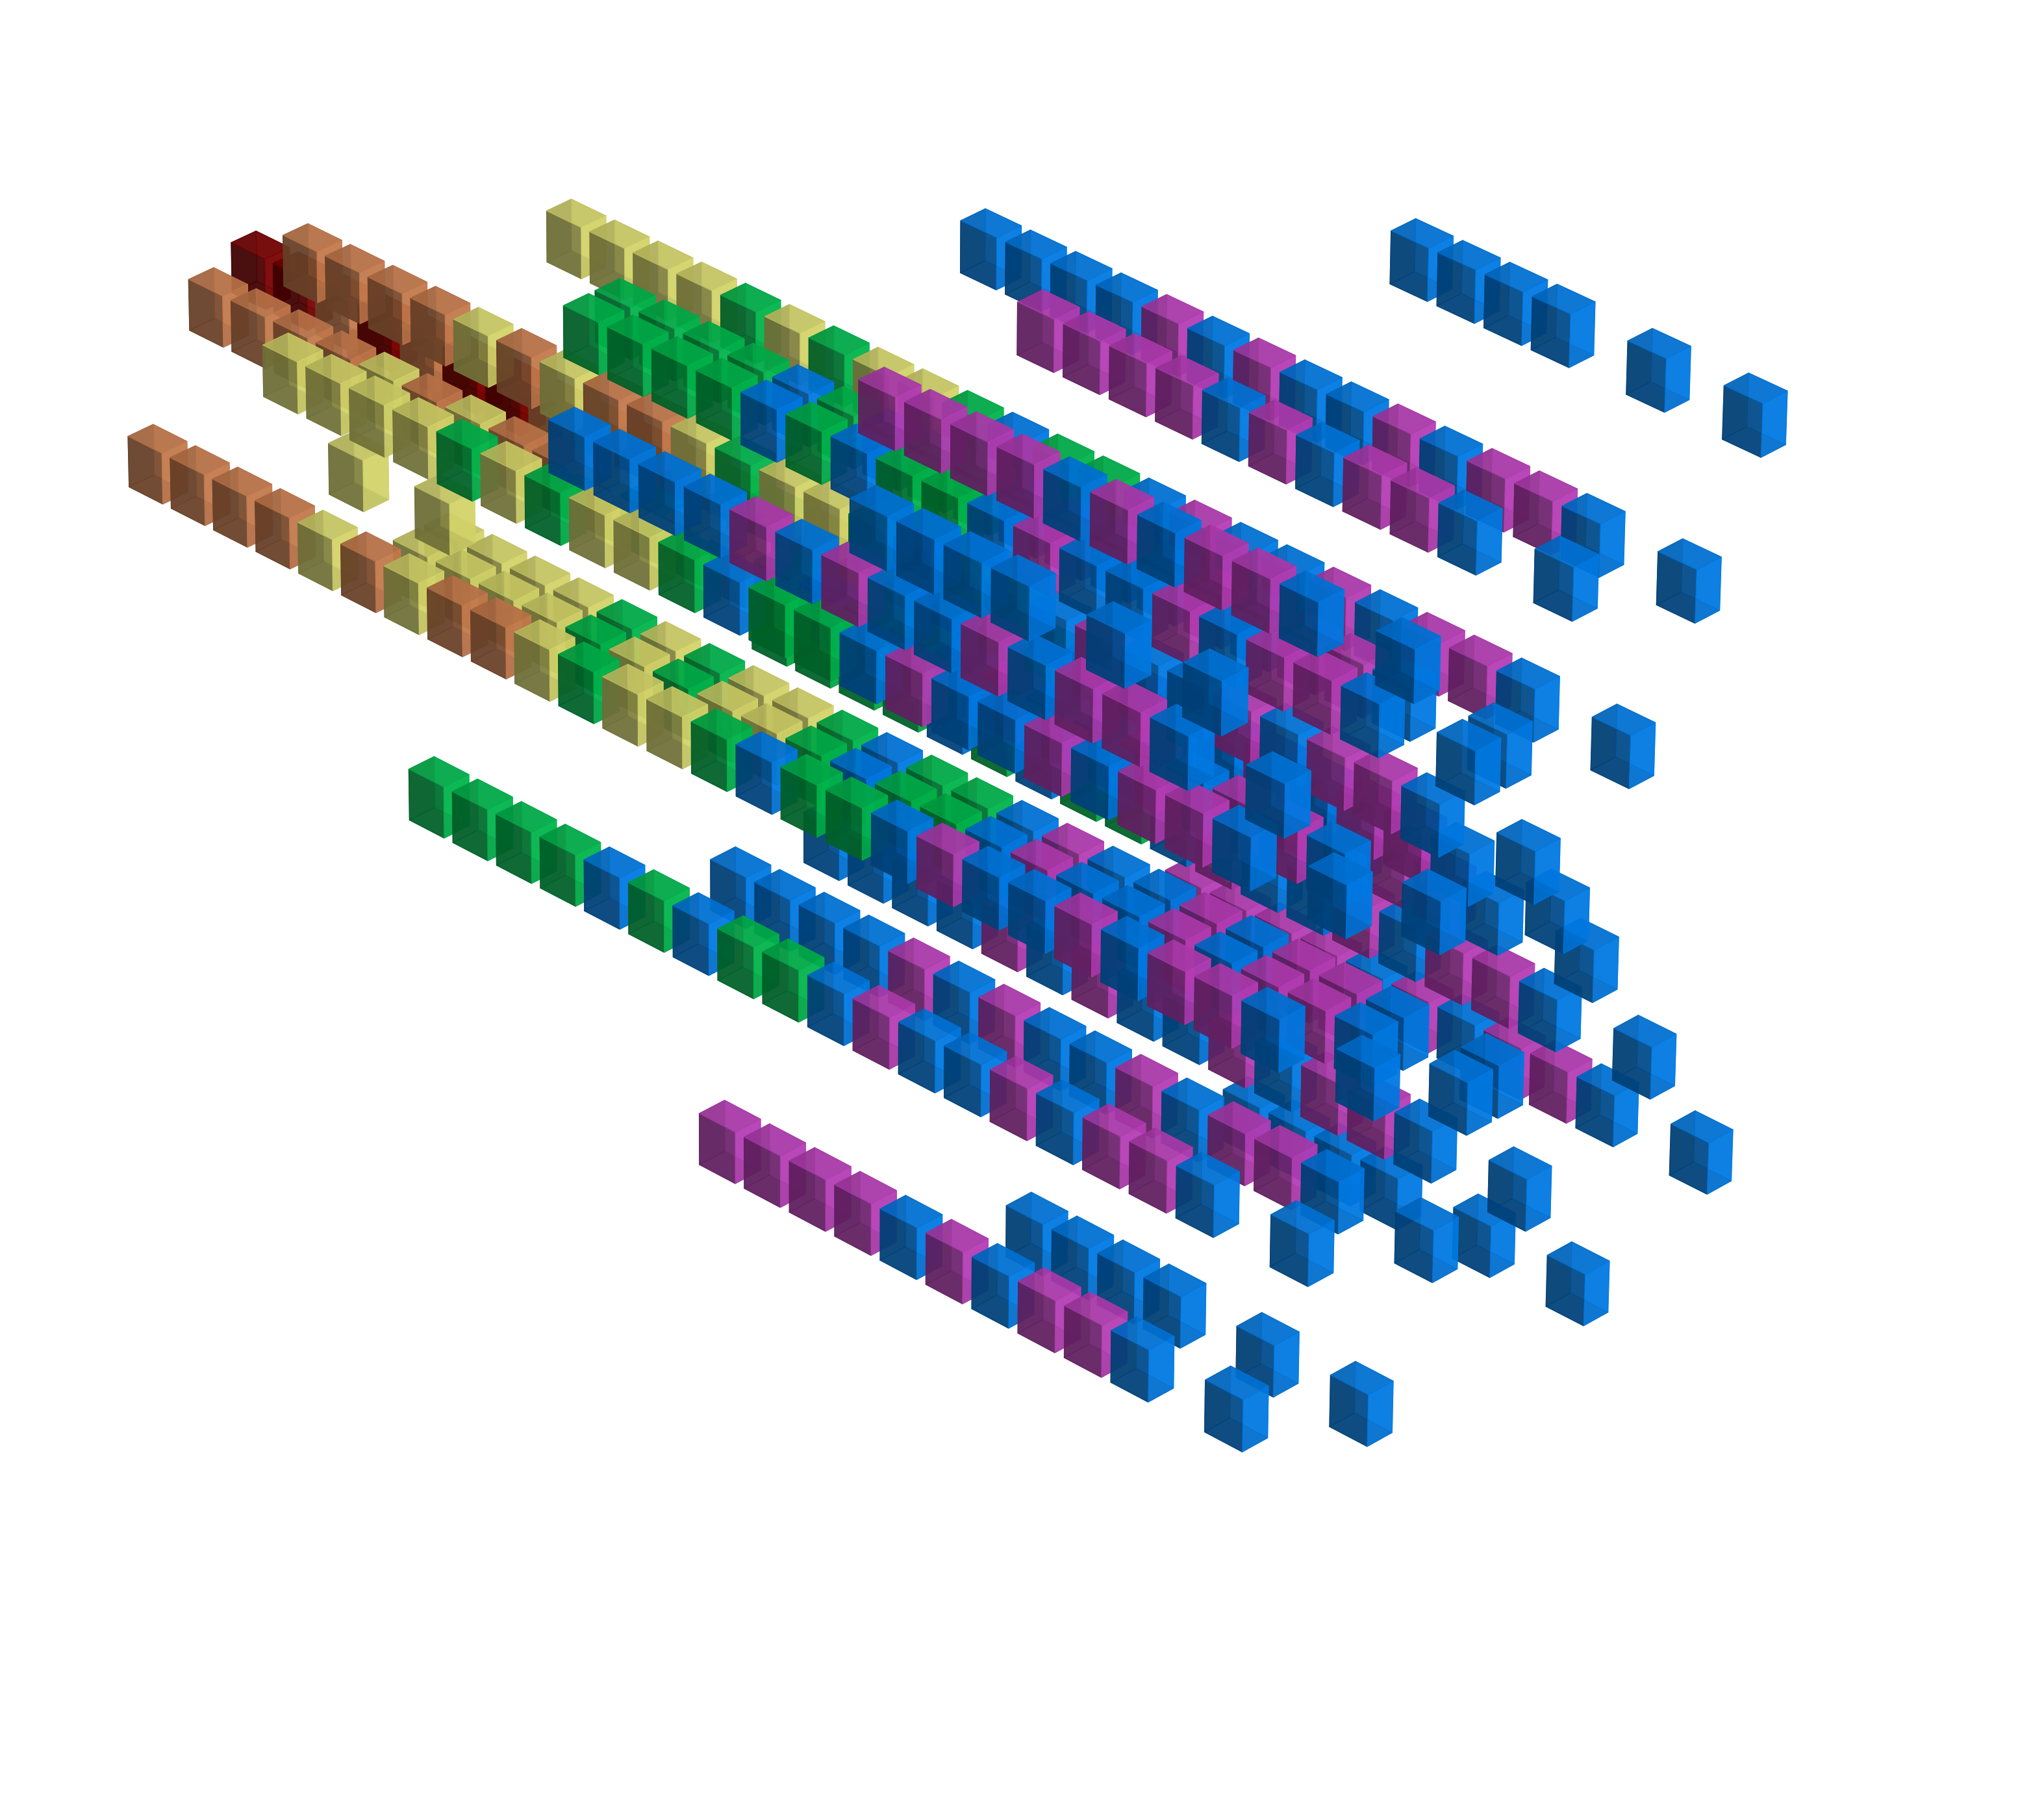
\includegraphics[width=11cm]{src/batalyx_patterns/pattern0-45.png}%
    \end{adjustbox}
    \begin{adjustbox}{width=11cm,margin=0cm -2cm}
      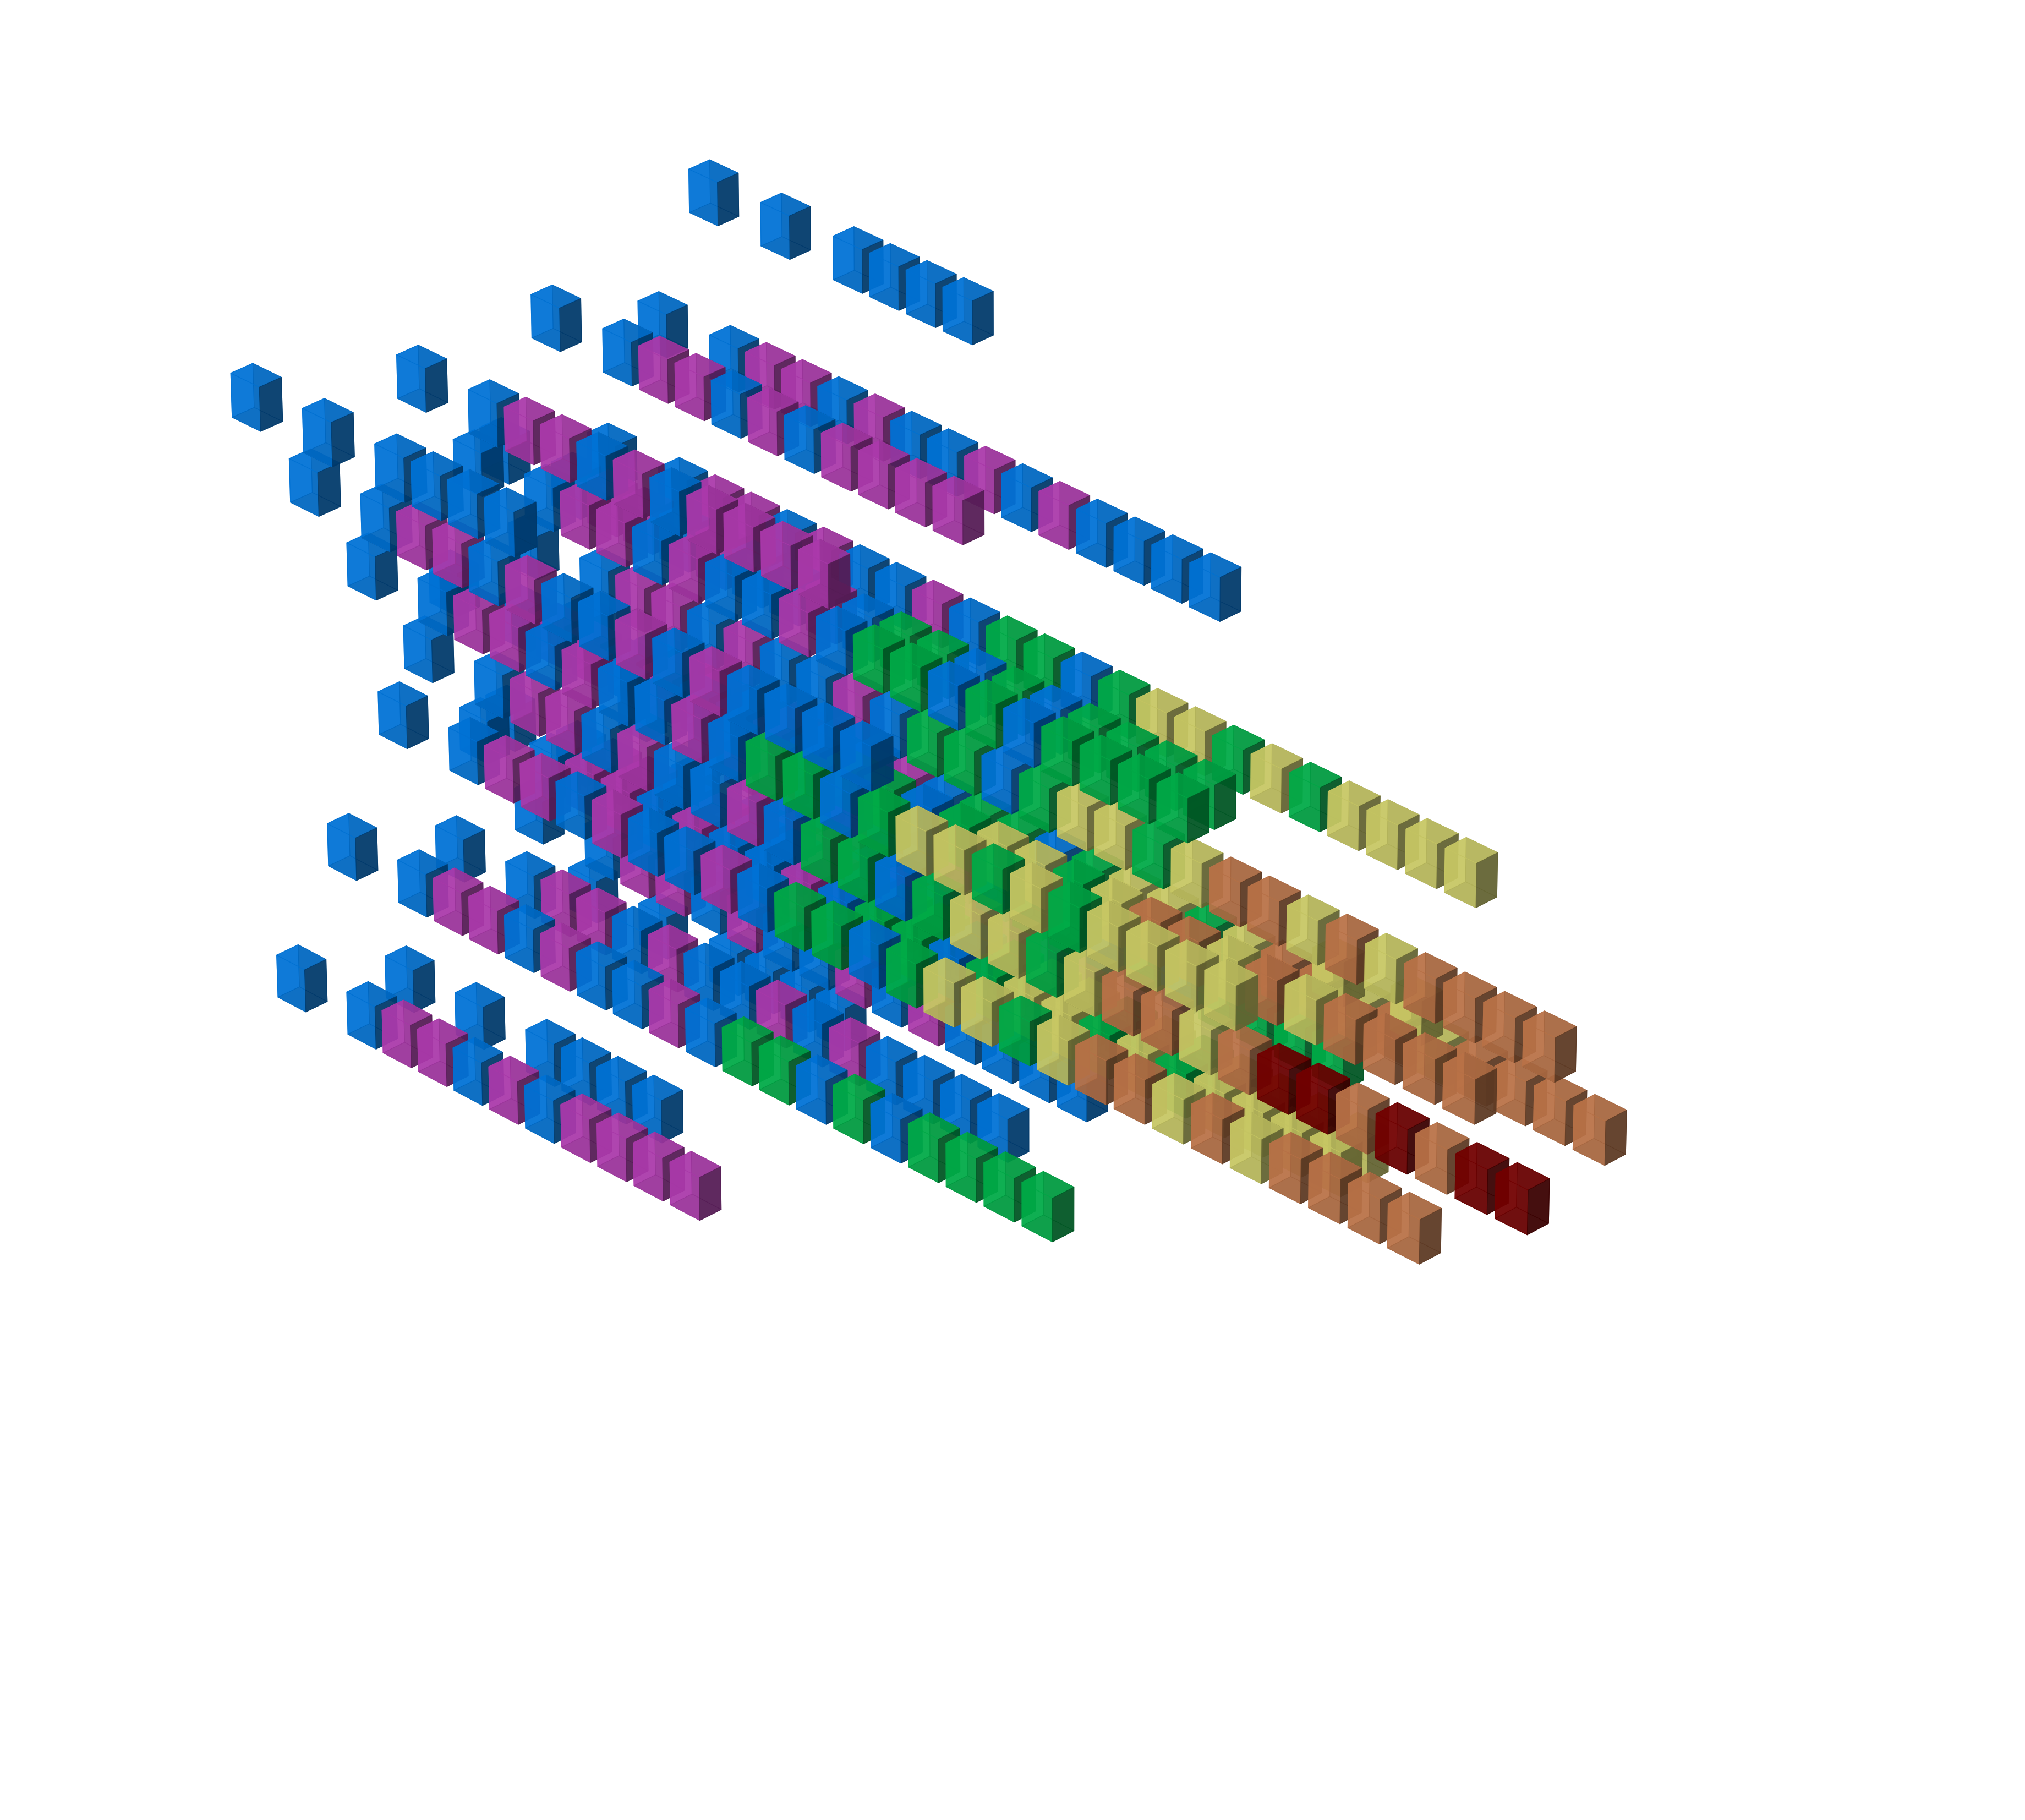
\includegraphics[width=11cm]{src/batalyx_patterns/pattern0-225.png}%
    \end{adjustbox}
\caption{Evolution of the 'Batalyx' pattern.}
\end{figure}

\rhead[]{Star One}
\begin{lstlisting}[caption=Source code for the Batalyx pattern..]
patternXPosArray             
        .BYTE $FF,$01,$55    ; 6              
        .BYTE $FE,$02,$55    ;            5   
        .BYTE $FD,$03,$55    ;   4            
        .BYTE $FC,$04,$55    ;          3     
        .BYTE $FB,$05,$55    ;     2          
        .BYTE $FA,$06,$55    ;        1       
        .BYTE $55,$55        ;                
patternYPosArray             ;      1         
        .BYTE $01,$FF,$55    ;         2      
        .BYTE $FE,$02,$55    ;    3           
        .BYTE $03,$FD,$55    ;           4    
        .BYTE $FC,$04,$55    ;  5             
        .BYTE $05,$FB,$55    ;             6 
        .BYTE $FA,$06,$55
        .BYTE $55,$55
\end{lstlisting}

\subfile{batalyx_patterns/tables/pattern0.tex}

\clearpage
\textbf{Lines 1189-1231. \icode{\textbf{LaunchPsychedelia}}} 
\begin{lstlisting}
;--------------------------------------------------------
; LaunchPsychedelia
;--------------------------------------------------------
LaunchPsychedelia
        SEI 
        JSR InitializePsychedelia
        JSR SetUpBackgroundPainting
        JSR InitializeColorIndexArray
        JSR InitializeStatusDisplayText
        JSR UpdateCurrentSettingsDisplay
        CLI 
PsychedeliaLoop   
        JSR MaybeUpdateFromBuffersAndPaint
        JSR CheckKeyboardInput
        JMP PsychedeliaLoop
\end{lstlisting}
\textbf{Lines 1189-1231. \icode{\textbf{MaybeUpdateFromBuffersAndPaint}}} 
\begin{lstlisting}[basicstyle=\ttfamily\scriptsize, caption=The routine responsible for painting patterns.]
MaybeUpdateFromBuffersAndPaint   
        LDX lastIndexToBuffers
        LDA currentColorIndexArray,X
        AND #$08
        BNE BufferUpdateComplete

        DEC smoothingDelayArray,X
        BNE BufferUpdateComplete

        LDA initialSmoothingDelayArray,X
        STA smoothingDelayArray,X

        LDA pixelXPositionArray,X
        STA currentPixelXPosition
        LDA pixelYPositionArray,X
        STA currentPixelYPosition

        LDA currentColorIndexArray,X
        STA currentColorIndex

        TAY 
        LDA symmetrySettingForStep,X
        STA currentSymmetrySettingForStep

        LDA presetColorValuesArray,Y
        STA currentColor

        INC currentColorIndexArray,X
        JSR PaintStructureAtCurrentPosition

BufferUpdateComplete   
        INC lastIndexToBuffers

        LDA lastIndexToBuffers
        AND #$3F
        STA lastIndexToBuffers
        RTS 
\end{lstlisting}
\clearpage

\rhead[]{\icode{LaunchPsychedelia}}
\textbf{Lines 1189-1231. \icode{\textbf{LaunchPsychedelia}}:} Psychedelia


\clearpage
\textbf{Lines 1189-1231. \icode{\textbf{PaintStructureAtCurrentPosition}}} 
\begin{lstlisting}[caption = All the pattern data structures in Psychedelia organized into a set of arrays.]
;--------------------------------------------------------
; PaintStructureAtCurrentPosition
;--------------------------------------------------------
PaintStructureAtCurrentPosition   
        LDA #$00
        STA currentPatternIndex
        STA currentLineInPattern

        LDA currentPixelXPosition
        STA initialPixelXPosition
        LDA currentPixelYPosition
        STA initialPixelYPosition

        JSR PaintPixelForCurrentSymmetry

        LDA currentColorIndex
        BNE PixelPaintLoop
        RTS 

PixelPaintLoop   
        LDX currentPatternIndex
        LDA patternXPosArray,X
        CMP #$55
        BEQ MoveToNextLineInPattern

        CLC 
        ADC currentPixelXPosition
        STA initialPixelXPosition

        LDA patternYPosArray,X
        CLC 
        ADC currentPixelYPosition
        STA initialPixelYPosition

        JSR PaintPixelForCurrentSymmetry

        INC currentPatternIndex
        JMP PixelPaintLoop

MoveToNextLineInPattern   
        INC currentPatternIndex
        INC currentLineInPattern
        LDA currentLineInPattern
        CMP currentColorIndex
        BNE PixelPaintLoop
        RTS 
\end{lstlisting}
\clearpage

\rhead[]{\icode{PaintStructureAtCurrentPosition}}
\textbf{Lines 1189-1231. \icode{\textbf{PaintStructureAtCurrentPosition}}:} Psychedelia

\clearpage
\textbf{Lines 1189-1231. \icode{\textbf{PaintPixelForCurrentSymmetry}}} 
\begin{lstlisting}[basicstyle=\ttfamily\scriptsize, caption=The routine responsible for painting patterns.]
;--------------------------------------------------------
; PaintPixelForCurrentSymmetry
;--------------------------------------------------------
PaintPixelForCurrentSymmetry   
        LDA initialPixelYPosition
        AND #$80
        BEQ CanPaintPixelOnThisLine

CleanUpAndReturn   
        RTS 

CanPaintPixelOnThisLine   
        LDA initialPixelYPosition
        CMP #TOP_Y_POSITION+1
        BPL CleanUpAndReturn

        LDA initialPixelXPosition
        AND #$80
        BNE CleanUpAndReturn

        LDA initialPixelXPosition
        CMP #NUM_COLS
        BPL CleanUpAndReturn

        LDA currentColor
        TAX 
        LDA colorComparisonArray,X
        STA lastColorValue
        DEC lastColorValue

        JSR PaintPixel

        LDA currentSymmetrySettingForStep
        BNE HasSymmetry

ReturnFromSymmetry   
        RTS 

\end{lstlisting}
\clearpage

\rhead[]{\icode{LaunchPsychedelia}}
\textbf{Lines 1189-1231. \icode{\textbf{LaunchPsychedelia}}:} Psychedelia

\clearpage
\textbf{Lines 1189-1231. \icode{\textbf{PaintPixelForCurrentSymmetry} continued.}} 
\begin{lstlisting}[caption = All the pattern data structures in Psychedelia organized into a set of arrays.]
HasSymmetry   
        CMP #X_Y_SYMMETRY
        BEQ HasXYSymmetry

        CMP #X_AXIS_SYMMETRY
        BEQ HasXAxisSymmetry

        LDA #NUM_COLS-1
        SEC 
        SBC initialPixelXPosition
        STA initialPixelXPosition

        JSR PaintPixel

        LDA currentSymmetrySettingForStep
        CMP #Y_AXIS_SYMMETRY
        BEQ ReturnFromSymmetry

        LDA #TOP_Y_POSITION
        SEC 
        SBC initialPixelYPosition
        STA initialPixelYPosition

        JSR PaintPixel

        LDA #NUM_COLS-1
        SEC 
        SBC initialPixelXPosition
        STA initialPixelXPosition

        JMP PaintPixel

HasXYSymmetry   
        LDA #TOP_Y_POSITION
        SEC 
        SBC initialPixelYPosition
        STA initialPixelYPosition

        JMP PaintPixel

HasXAxisSymmetry   
        LDA #NUM_COLS-1
        SEC 
        SBC initialPixelXPosition
        STA initialPixelXPosition
        JMP HasXYSymmetry
\end{lstlisting}
\clearpage

\rhead[]{\icode{LaunchPsychedelia}}
\textbf{Lines 1189-1231. \icode{\textbf{LaunchPsychedelia}}:} Psychedelia
\clearpage
\textbf{Lines 1189-1231. \icode{\textbf{PaintPixel}}} 
\begin{lstlisting}[caption = All the pattern data structures in Psychedelia organized into a set of arrays.]
;--------------------------------------------------------
; PaintPixel
;--------------------------------------------------------
PaintPixel   
        LDX initialPixelYPosition
        LDY initialPixelXPosition
        LDA screenLinesLoPtrArray,X
        STA colorRAMLoPtr
        LDA screenLinesHiPtrArray,X
        CLC 
        ADC #OFFSET_TO_COLOR_RAM
        STA colorRAMHiPtr
        LDA (colorRAMLoPtr),Y
        AND #$0F
        CMP currentColorValue
        BEQ ActuallyPaintPixel

        TAX 
        LDA colorComparisonArray,X
        CMP lastColorValue
        BEQ ActuallyPaintPixel
        BPL ActuallyPaintPixel
        RTS 

ActuallyPaintPixel   
        LDA currentColor
        STA (colorRAMLoPtr),Y
        RTS 

colorComparisonArray   
        .BYTE ORANGE,ORANGE,WHITE,ORANGE,BLUE,PURPLE,YELLOW,CYAN
        .BYTE RED,ORANGE,ORANGE,ORANGE,ORANGE,ORANGE,GREEN,ORANGE
        .BYTE ORANGE

\end{lstlisting}
\clearpage

\rhead[]{\icode{LaunchPsychedelia}}
\textbf{Lines 1189-1231. \icode{\textbf{LaunchPsychedelia}}:} Psychedelia
